\begin{figure}[!ht]
    \centering

\tikzset{every picture/.style={line width=0.75pt}} %set default line width to 0.75pt        
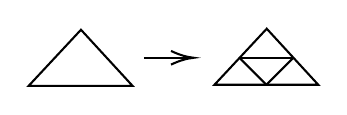
\begin{tikzpicture}[x=0.75pt,y=0.75pt,yscale=-1,xscale=1]
%uncomment if require: \path (0,300); %set diagram left start at 0, and has height of 300

%Shape: Triangle [id:dp5526310537518102] 
\draw   (184.18,86.13) -- (209,113.13) -- (159,113.13) -- cycle ;
%Straight Lines [id:da5309512728134356] 
\draw    (184,113.13) -- (171,100.13) ;
%Straight Lines [id:da318567472926536] 
\draw    (171,100.13) -- (197,100.13) ;
%Straight Lines [id:da5008865323179771] 
\draw    (184,113.13) -- (197,100.13) ;
%Shape: Triangle [id:dp3052310642312507] 
\draw   (94.68,86.63) -- (119.5,113.63) -- (69.5,113.63) -- cycle ;
%Straight Lines [id:da020905912975204166] 
\draw    (125,100.13) -- (147,100.13) ;
\draw [shift={(149,100.13)}, rotate = 180] [color={rgb, 255:red, 0; green, 0; blue, 0 }  ][line width=0.75]    (10.93,-3.29) .. controls (6.95,-1.4) and (3.31,-0.3) .. (0,0) .. controls (3.31,0.3) and (6.95,1.4) .. (10.93,3.29)   ;

\end{tikzpicture}
    \caption{Multi-mesh face division}
    \label{fig:mesh-face}
\end{figure}